\documentclass[12pt, a4paper]{article}

% Preamble with packages
\usepackage{graphicx}
%\usepackage{amsmath}
\usepackage[hidelinks]{hyperref}
%\usepackage{url}
\usepackage{listings} % Required for typesetting code
% \hypersetup{breaklinks=true} % Vill inte att hela sida 9 ska bli en länk...

\lstnewenvironment{sqlCode}
    {\lstset{language=SQL, % Set language to SQL
             basicstyle=\ttfamily, % Use typewriter font
             keywordstyle=\bfseries, % Use bold for keywords
             commentstyle=\itshape, % Use italics for comments
             columns=fullflexible, % Allow flexible column formatting
             flexiblecolumns=true, % Enable flexible column formatting
             showstringspaces=false, % Don't show spaces in strings
            % frame=single, % Draw a frame around the code
            % rulecolor=\color{gray}, % Set the frame color to grey
             }}
    {}


% Set the title
\title{Graph Databases: A Comparative Study with Relational Models}
\author{
  Max Rydberg, Erik Björnlinger \\
  \texttt{gusrydmaac@student.gu.se, guseribj@student.gu.se} \\
  Computer Science Department, University of Gothenburg 
}
\date{\today}


% Begin the document
\begin{document}

\maketitle

\begin{abstract}
This study explores the performance and application differences between graph databases and traditional relational databases. Using Neo4j and PostgreSQL, we demonstrate the advantages of each model through a series of tests on diverse datasets. Our findings suggest that while graph databases offer superior performance for complex query environments, relational databases remain effective for structured data applications.

\end{abstract}

\section{Introduction}
The landscape of database technologies has evolved significantly over the past few decades. Traditionally, relational databases, based on the relational model introduced by E.F. Codd\footnote{E.F. Codd, "A Relational Model of Data for Large Shared Data Banks," \textit{Communications of the ACM}, vol. 13, no. 6, pp. 377-387, 1970. Available: \url{https://cs.uwaterloo.ca/~david/cs848s14/codd-relational.pdf}} in the 1970s, have been the cornerstone of data storage and management. These databases organize data into tables with predefined schemas, making them suitable for structured data and transactional applications. However, during the 2000s, the rise of web-scale applications, social networks, and big data exposed the limitations of relational databases in handling highly interconnected and dynamic data.

Graph databases have emerged as a powerful alternative to relational databases for managing complex and interconnected datasets. Unlike relational databases, graph databases model data as nodes (entities) and edges (relationships), allowing for more natural and flexible data representation. This approach is particularly effective for applications that require traversing relationships, such as social networks, recommendation systems, and fraud detection.

Despite the growing interest in graph databases, there is still a need for a comprehensive comparison with traditional relational databases to understand their respective strengths and limitations. Developers and data scientists often face challenges in selecting the appropriate database technology for their specific needs, especially when dealing with complex data structures and relationships.

The primary objective of this paper is to provide a comparative study between graph databases and relational databases. Using Neo4j as a representative of graph databases and PostgreSQL as a representative of relational databases, we aim to evaluate their performance, efficiency, and suitability for different types of applications.


This paper is structured as follows:
\begin{itemize}
    \item \textbf{Section 2:} An overview of graph databases, including their types and unique characteristics.
    \item \textbf{Section 3:} A detailed comparison between graph databases and relational databases, focusing on paradigm differences, query languages, and data modeling.
    \item \textbf{Section 4:} A discussion of related work, highlighting existing research and studies on this topic.
    \item \textbf{Section 5:} A summary of the key findings from the comparative study.
    \item \textbf{Section 6:} Our conclusions and suggestions for future work.
\end{itemize}


\section{What are Graph Databases?}
Graph databases are a type of NoSQL database designed to store, manage, and query data that is highly interconnected. Unlike traditional relational databases, which organize data in tables, graph databases represent data as a graph composed of nodes, edges, and properties.

\textbf{Nodes:} These represent entities or objects in the database, such as people, places, or items.

\textbf{Edges:} These define relationships between nodes. For instance, an edge can represent a ``friendship'' relationship between two nodes representing people.

\textbf{Properties:} Both nodes and edges can have properties, which are key-value pairs that provide additional information about the nodes and edges. For example, a node representing a person might have properties like ``name'' and ``age,'' while an edge representing a friendship might have a property ``since'' indicating when the friendship started.

Graph databases are particularly powerful for applications that involve complex relationships and dynamic schemas. Examples include social networks, recommendation systems, and fraud detection systems.

\subsection{Types of Graph Databases}

Graph databases can be implemented using different underlying concepts for representing data. The two most common such concepts in graph databases are RDF (Resource Description Framework) and LPG (Labeled Property Graphs).\footnote{Angels, R. (2012) A Comparison of Current Graph Database Models. 2012 IEEE 28th International Conference on Data Engineering Workshops}
Both RDF and LPG use a graph as its underlying concept but differs in how the data is stored in the graph. RDF uses a triple of a subject, predicate and object, all encapsulated in URLs as their underlying data structure (see Figure 1). 
\begin{figure}[H]
  \centering
  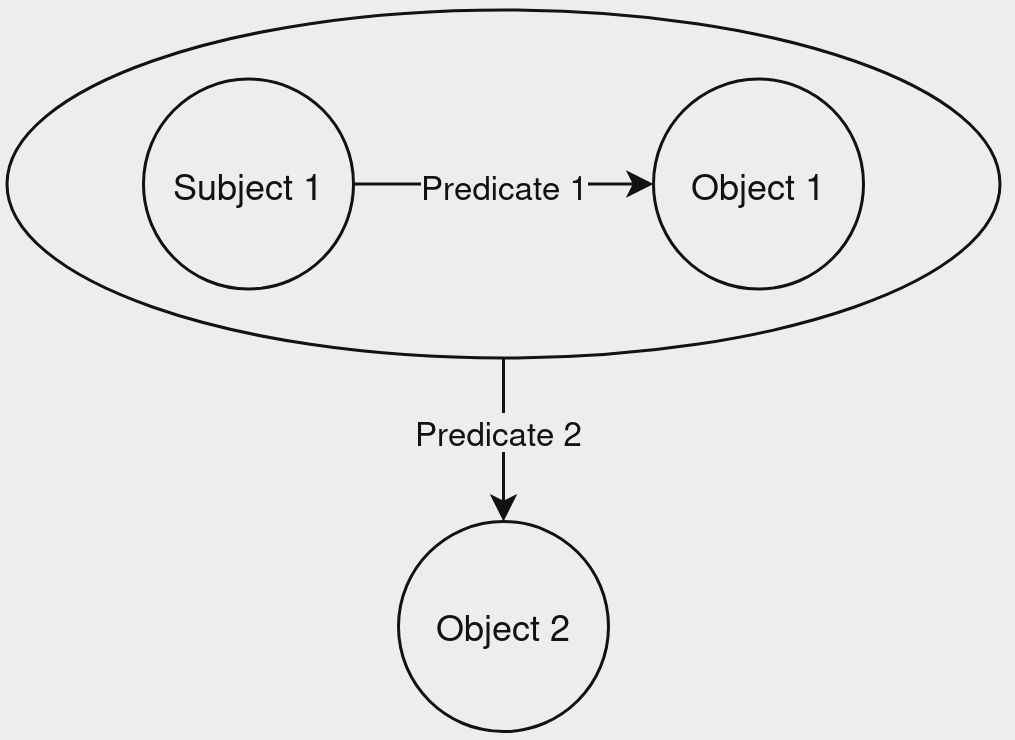
\includegraphics[width=0.5\textwidth]{assets/RDF-example.png}
  \caption{A simple RDF structure}
\end{figure}
The subject is the resource that is being described, the predicate is a property or characteristics of the subject and the object is the value of the property. Because all data is encapsulated in URLs RDF is useful when the represented data is already in the form of an URL. Meaning that when the data is in the web an RDF database could be useful. The subject, the predicate and the value do not have attributes or associated key value pairs. In order to add information about the relationships the subject in a triple of subject, predicate and object, has to be a triple itself. 

In LPG the data is represented in the nodes and the edges between the nodes. The entities, or nouns, are represented as nodes and the relationships between the entities are represented in the edges (see Figure 2). 
\begin{figure}[H]
  \centering
  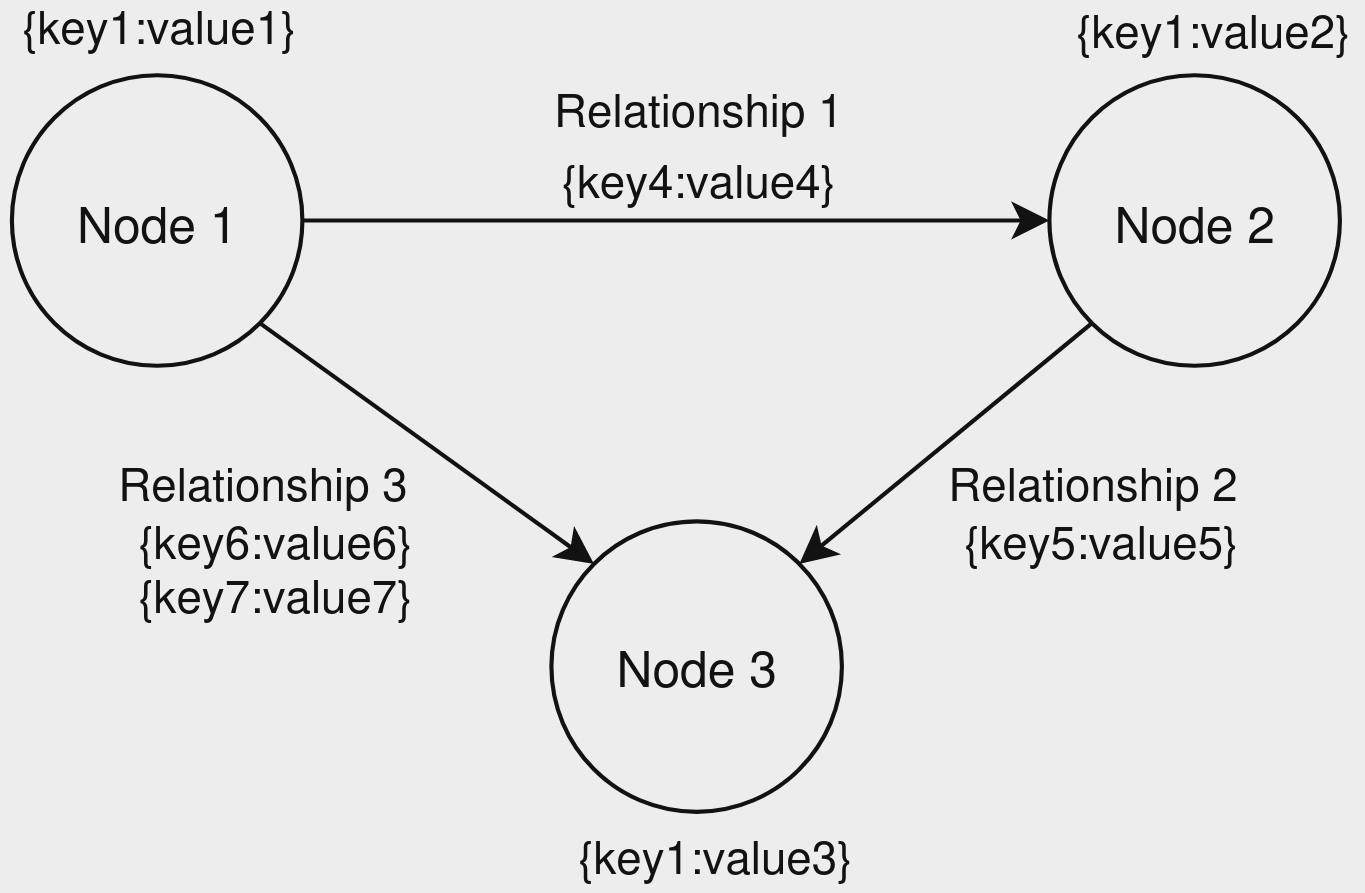
\includegraphics[width=0.5\textwidth]{assets/LPG-example.png}
  \caption{A simple LPG structure}
\end{figure}
Both the nodes and the edges can be labeled with attributes about the entity or the relationship. Attributes are specified in a key value structure. An attributes about a relationship between two entities is therefore specified in the relation itself. Neo4j is a graph database that has LPG as it's underlying concept.\footnote{Angels, R. (2012) A Comparison of Current Graph Database Models. 2012 IEEE 28th International Conference on Data Engineering Workshops}

\subsection{Key Features of Graph Databases}

\textbf{1. Schema-Free:} Graph databases are typically schema-free, meaning the data model can evolve without the need for predefined schemas. This flexibility allows for easier adjustments and scalability as data and relationships grow.

\textbf{2. Efficient Relationship Handling:} Graph databases excel at managing and querying complex relationships.\footnote{López, F.M.S., De La Cruz E. G. S. (2015) Literature review about Neo4j graph database as a feasible alternative for replacing RDBMS. Network of Scientific Journals from Latin America, the Caribbean, Spain and Portugal} Traversing relationships in a graph database is more efficient than performing multiple joins in a relational database.

\textbf{3. Query Languages:} Graph databases use specialized query languages designed for graph traversal and pattern matching. The most notable query language for graph databases is Cypher, used by Neo4j. Cypher provides a syntax that is easy to learn and allows for expressive and efficient graph queries.



% Cypher and Neo4j will be used as examples in the comparison with relational databases. Some knowledge of SQL is expected to understand the concepts discussed in this paper.

% % tables vs graphs, show an image of a table and a graph
% % add image from assets filder
% \begin{figure}[ht]
%     \centering
%     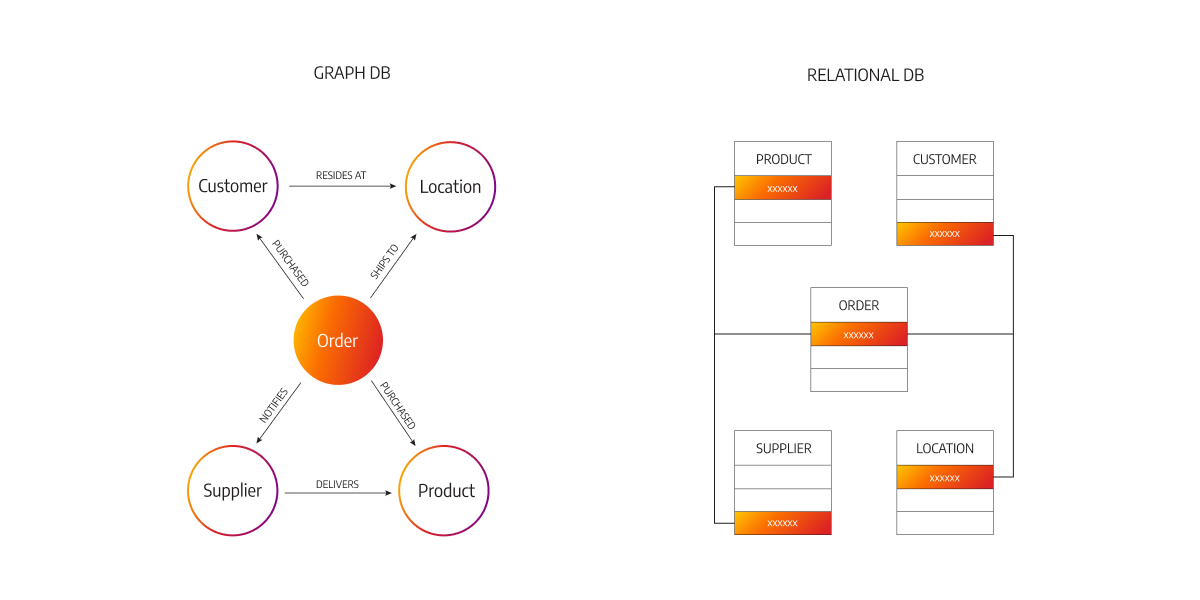
\includegraphics[width=0.7\textwidth]{assets/memgraph-graph-database-vs-relational-database.png}
%     \caption{Comparison of graph databases vs. relational databases.\protect\footnote{Image source: Memgraph, \url{https://memgraph.com/blog/graph-database-vs-relational-database}}}
%     \label{fig:graph_vs_table}
% \end{figure}
% In Figure \ref{fig:graph_vs_table}, we see a comparison of graph databases and relational databases. The graph database on the left shows a graph schema, while the relational database on the right shows a relational schema. The graph schema shows nodes and relationships between nodes, while the relational schema shows tables and relationships between tables. 

% \begin{figure}[ht]
%     \centering
%     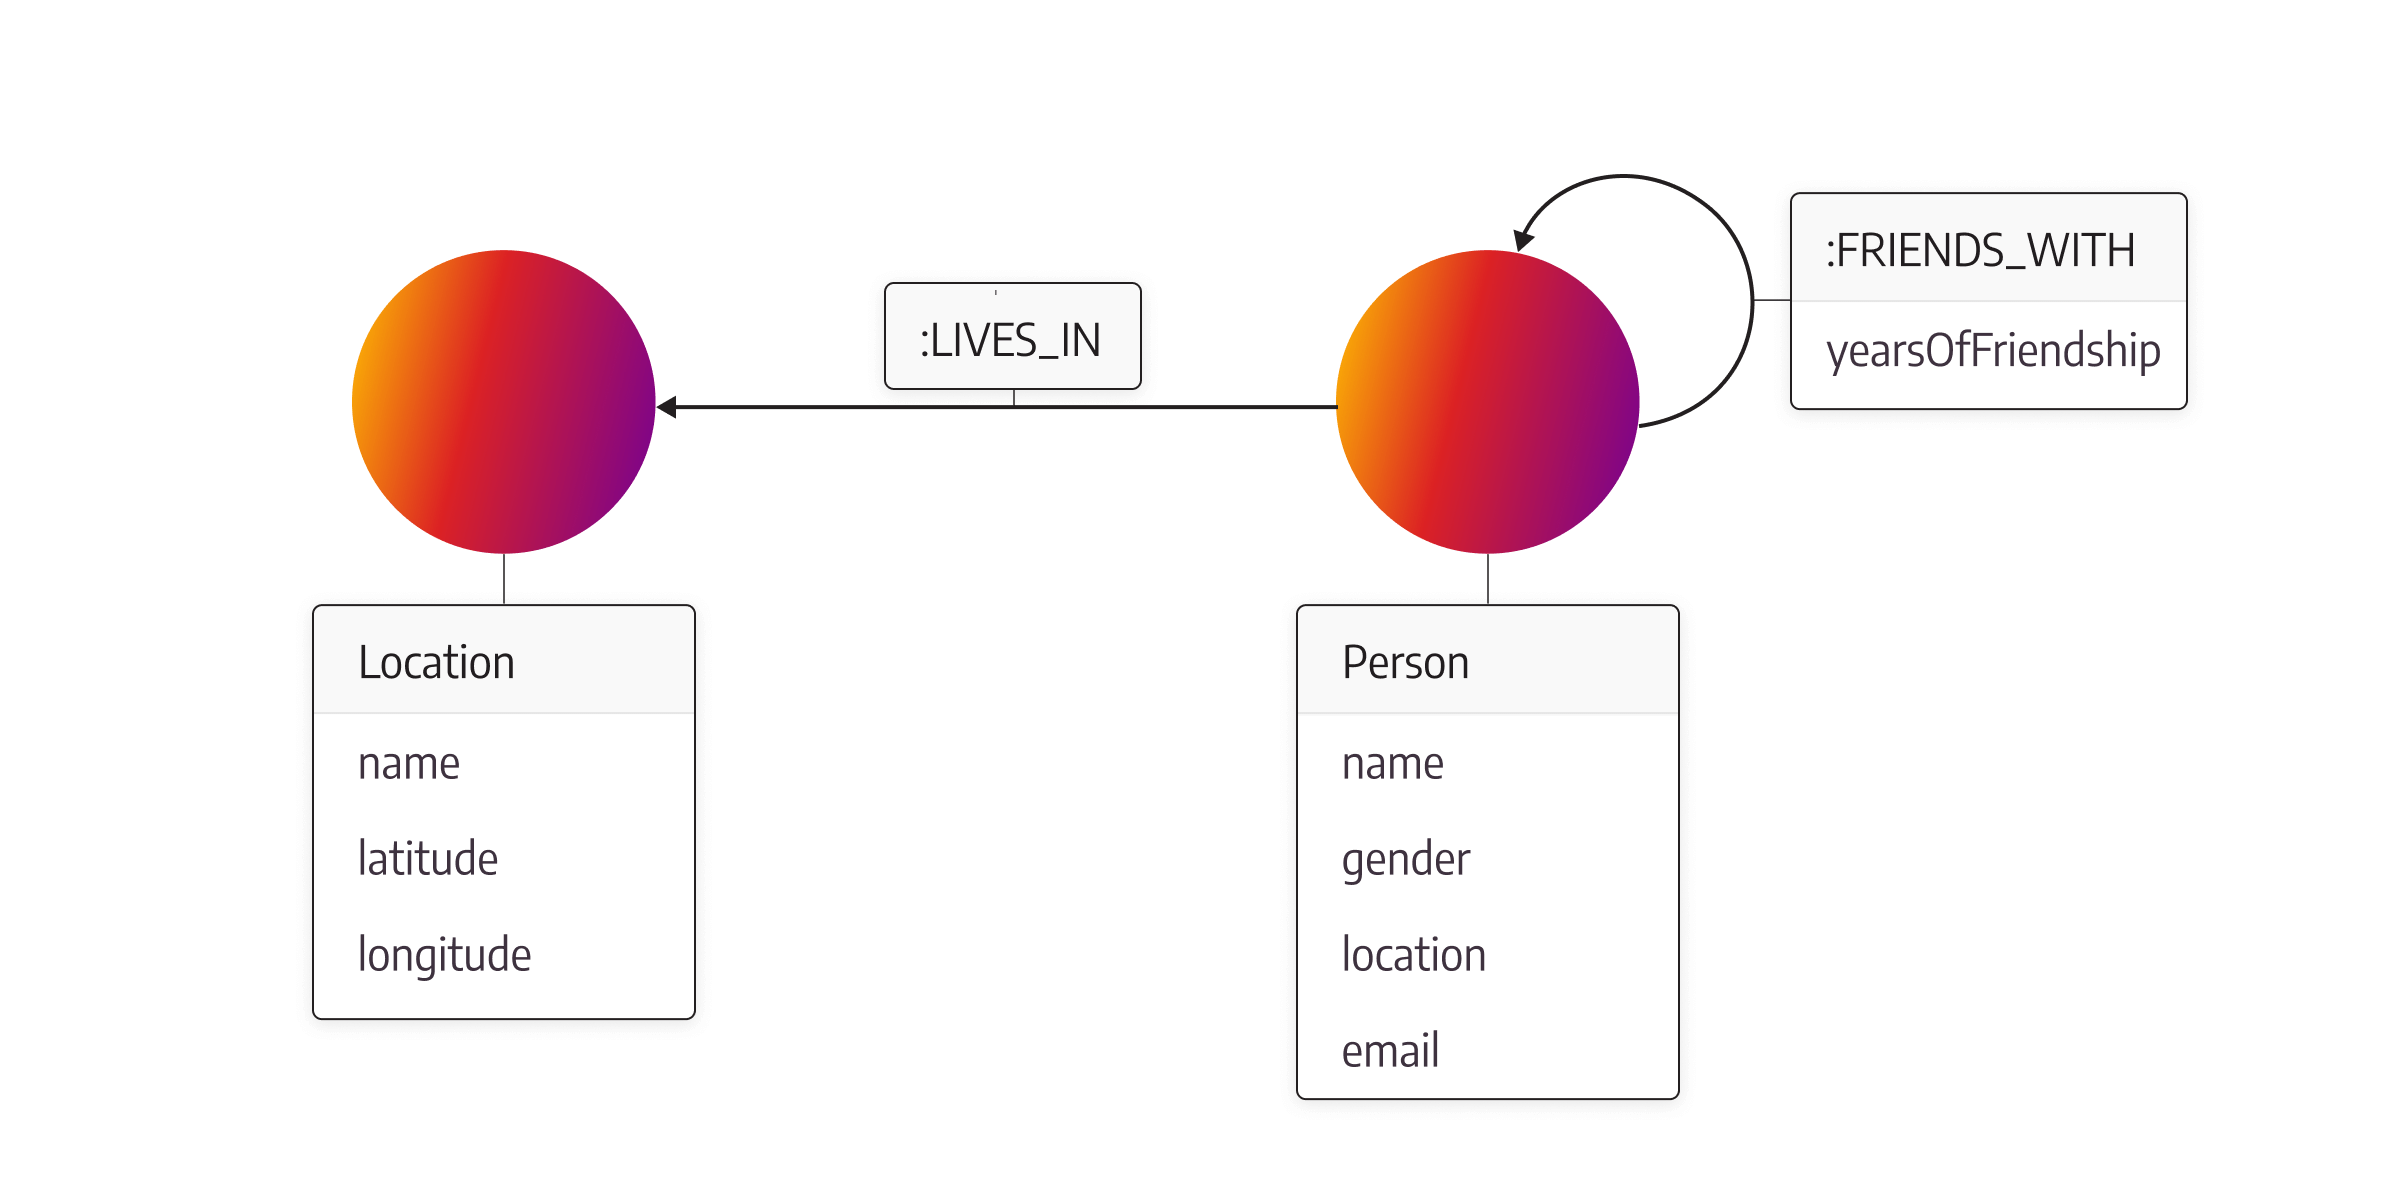
\includegraphics[width=0.7\textwidth]{assets/memgraph-graph-schema.png}
%     \caption{Graph Schema.\protect\footnote{Image source: Memgraph, \url{https://memgraph.com/blog/graph-database-vs-relational-database}}}
%     \label{fig:graph_schema}
% \end{figure}
% In Figure \ref{fig:graph_schema}, we see a graph schema. The graph schema shows nodes and relationships between nodes. The nodes represent entities, while the relationships represent the connections between entities. 

% \begin{figure}[ht]
%     \centering
%     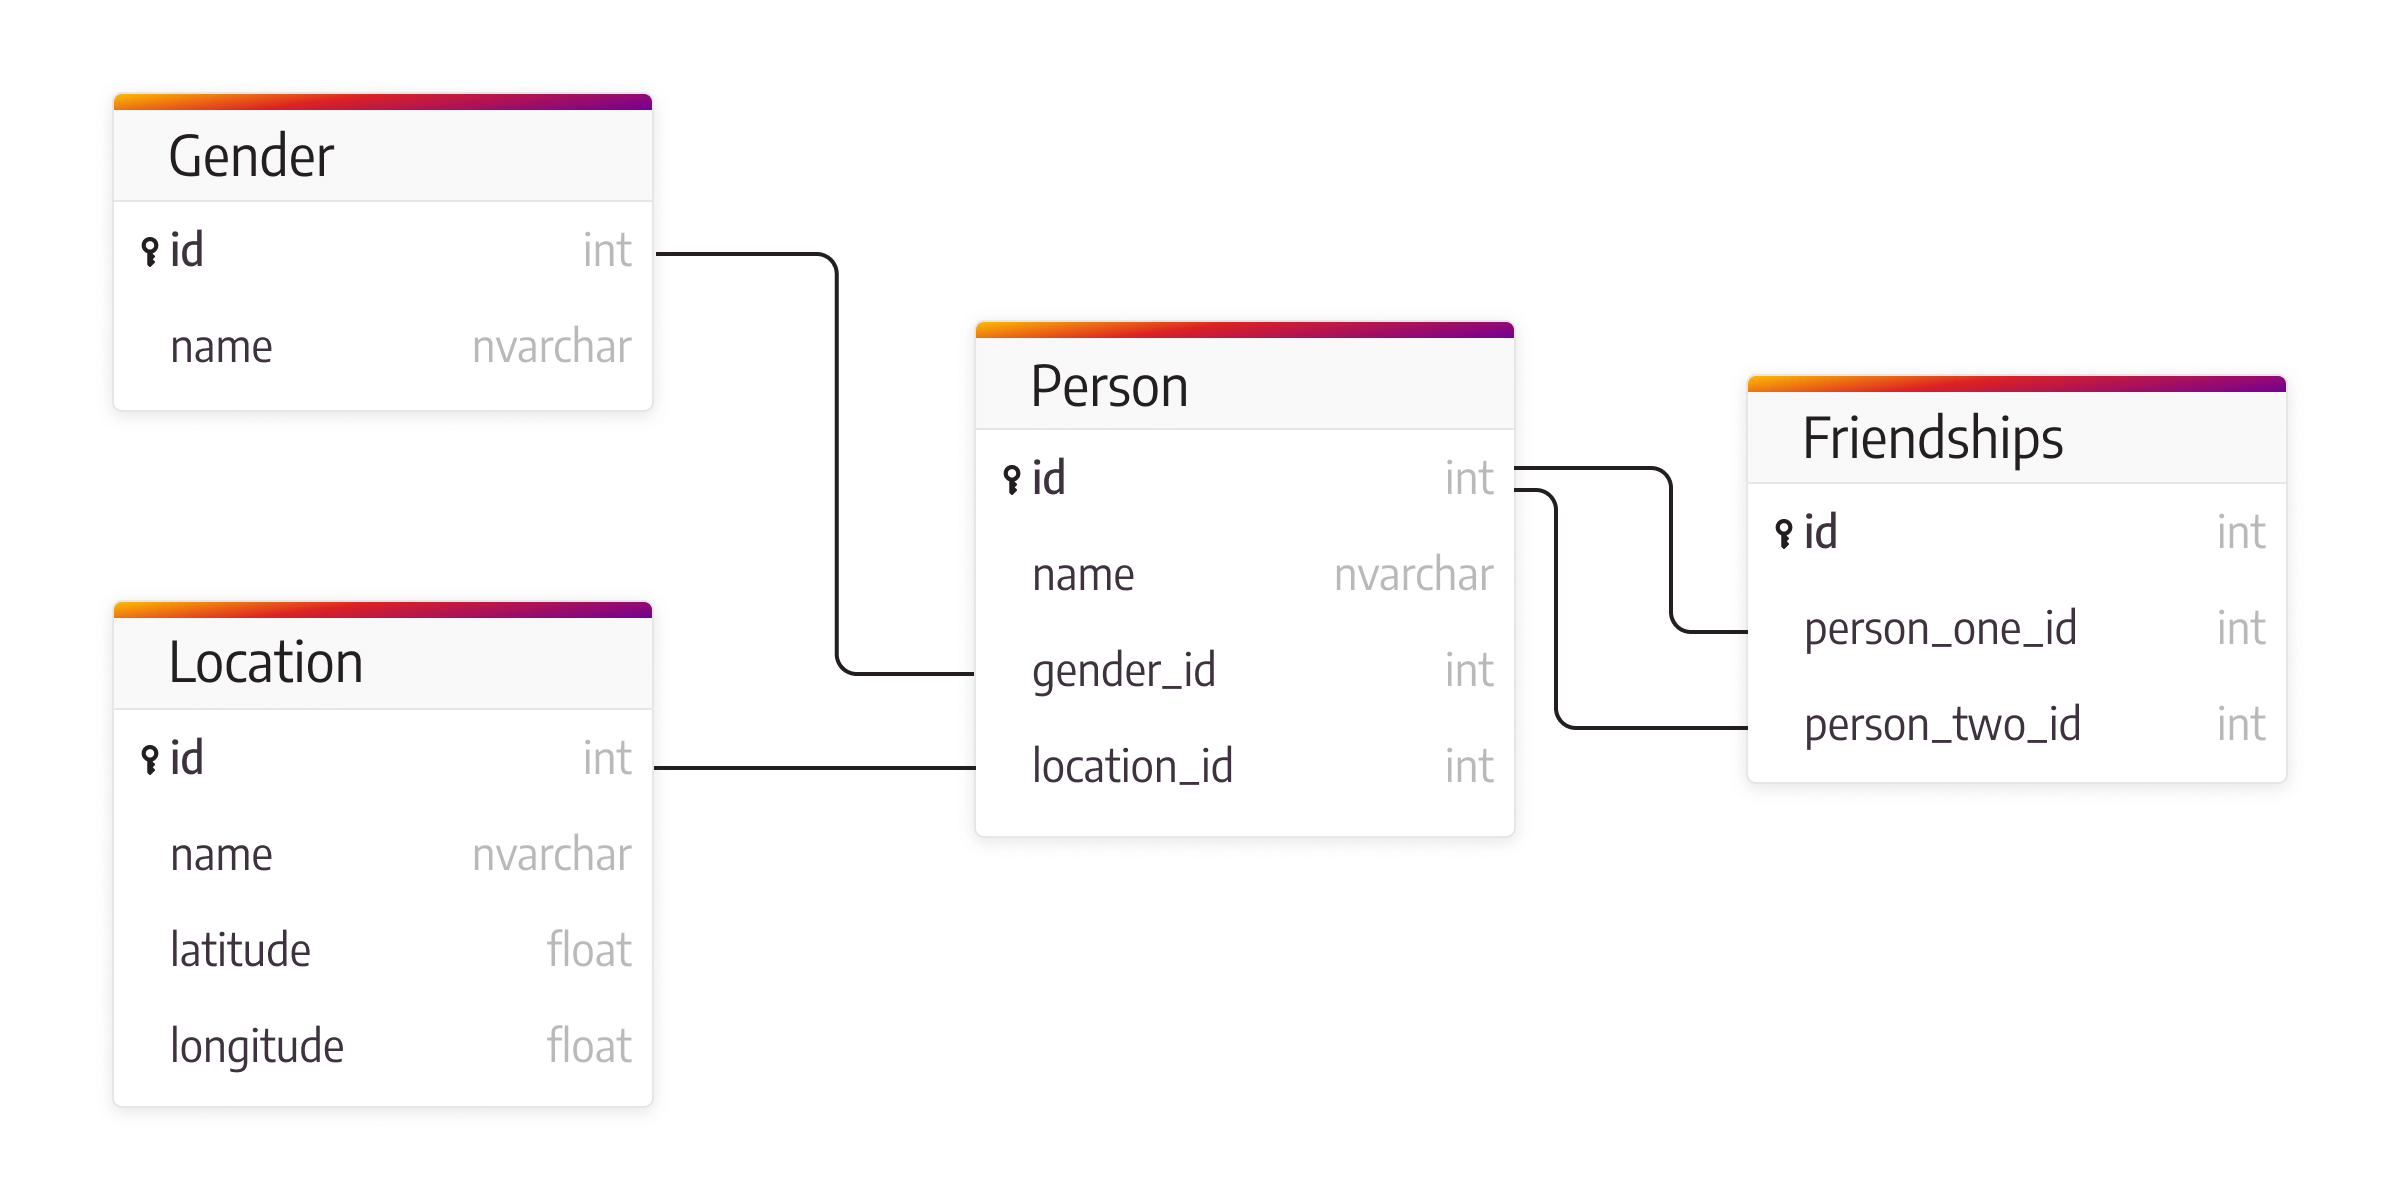
\includegraphics[width=0.7\textwidth]{assets/memgraph-relational-schema.png}
%     \caption{Relational Schema.\protect\footnote{Image source: Memgraph, \url{https://memgraph.com/blog/graph-database-vs-relational-database}}}
%     \label{fig:relational_schema}
% \end{figure}
% In Figure \ref{fig:relational_schema}, we see a relational schema. The relational schema shows tables and relationships between tables. The tables represent entities, while the relationships represent the connections between entities.

\subsection{An example in Cypher and SQL}
In order to highlight the potential that graph databases offers, we will in this section look at a few examples queries in SQL (Structured Query Language) and in Cypher. 
As mention above, Neo4j does not use standard SQL for interacting with the database. Instead it uses a query-language called Cypher. Cypher is a declarative language that has a similar syntax to SQL. Because Cypher is used when interacting with graph databases it offers some functionality not found in SQL. The syntax in Cypher is visual in nature as a node in Cypher are expressed within parenthesis and a relation is expressed within square brackets. A query containing both nodes and relationships can therefore be seen as a small graph with labeled edges. Let us look at some examples in Cypher and compare them with the corresponding SQL. The following Cypher examples are from the official documentation for Neo4j. \footnote{Neo4j docs - Basic queries 2024-05-20 \url{https://neo4j.com/docs/cypher-manual/current/queries/basic/}} In these examples we assume that we already have a database that contains information regarding actors and movies. Here is an example query in Cypher:
\begin{sqlCode}
  MATCH (keanu:Person {name:'Keanu Reeves'})
  RETURN keanu.name AS name, keanu.born AS born
\end{sqlCode}
Here we query the database after a node that has the property name 'Keanu Reeves', if we find such a node we return a table with that nodes \texttt{name} and \texttt{born} properties. The table would look like this:
\begin{center}
  \begin{tabular}{|c|c|}
    \hline
    name           & born \\
    \hline
    "Keanu Reeves" & 1964 \\
    \hline
  \end{tabular}\\
\end{center}
Here is a SQL query that would return a similar table from a relational database:


\begin{sqlCode}
SELECT
  name AS name,
  born AS born
FROM
  Person
WHERE
  name = 'Keanu Reeves';
\end{sqlCode}

For simple queries as the ones above there are little to no difference between Cypher and SQL. However some kind of queries are better suited for graph databases. Such queries are for example when the information that we want to find out is not necessarily structured inside the database. Let us look at an example, here is a query that finds if there is any direct or indirect relation between two actors and returns the shortest path if such a relation exist:

\begin{sqlCode}
MATCH p=shortestPath(
(:Person {name:"Keanu Reeves"})-[*]-(:Person{name:"Tom Hanks"})
) RETURN p
\end{sqlCode}

The query above can be read as; find the shortest path between the node with the name property "Keanu Reeves" and a the node with the name property "Tom Hanks". The inner query returns all relation of any length between the two nodes and the function \texttt{shortestPath()} returns the shortest relation between them. The \texttt{-[*]-} between the two nodes matches all direct and indirect relations between them. An similar query in SQL could be constructed the following way:
\begin{sqlCode}
WITH RECURSIVE ShortestPath AS (
SELECT
  id,
  name,
  ARRAY[id] AS path,
  0 AS depth
FROM
  people
WHERE
  name = 'Keanu Reeves'

UNION ALL

SELECT
  p.id,
  p.name,
  sp.path || p.id,
  sp.depth + 1
FROM
  ShortestPath sp
JOIN
  relationships r ON sp.id = r.person1_id
JOIN
  people p ON r.person2_id = p.id
WHERE
  NOT p.id = ANY(sp.path)
  )
SELECT *
FROM ShortestPath
WHERE name = 'Tom Hanks'
ORDER BY depth
LIMIT 1;

\end{sqlCode}
In this query we have to use a recursive common table expression in order to achieve the same functionality as in the Cypher query. This example shows that some functionality in relational database require more complexity from the query language. The difference in length between the two queries shows the difference in complexity. Queries of this nature is where graph databases are more appropriate to use rather than relational databases. The specifics of the database that is being queried and how much data that is in said database does impact the efficiency of the queries, but less complexity is often preferable when interacting with databases.





\section{Paradigm Differences}
Graph databases, such as Neo4j, and relational databases, such as PostgreSQL, differ significantly in their data models, query languages, performance characteristics, and suitable use cases. These differences stem from their foundational design principles, making each type of database optimal for different scenarios.

The following section compares graph databases and relational databases. The discussion is inspired by insights from several sources, including Analytics Vidhya, Neo4j documentation, and the DEV Community\footnote{Relational Database vs Graph Database: A Comparison Guide - Analytics Vidhya. \url{https://www.analyticsvidhya.com/blog/2021/05/relational-database-vs-graph-database-a-comparison-guide/}}\footnote{Graph Database vs. Relational Database (RDBMS) Model Comparison - Neo4j. \url{https://neo4j.com/developer/graph-database-vs-rdbms/}}\footnote{Relational Databases vs Graph Databases: A Comparison - DEV Community. \url{https://dev.to/anzaytuna/relational-databases-vs-graph-databases-a-comparison-28mj}}.

\textbf{Data Models:} Relational databases organize data into tables with predefined schemas, where each table represents an entity, and relationships between entities are managed using foreign keys. This tabular structure is efficient for structured data and well-defined relationships but can become cumbersome when handling complex interconnections. Conversely, graph databases use nodes to represent entities and edges to represent relationships, allowing for a more natural and flexible representation of interconnected data. This model is particularly advantageous for applications involving complex relationships and dynamic schemas.

\textbf{Query Languages:} Relational databases use SQL (Structured Query Language) for data management and querying. SQL is powerful for operations involving structured data and multiple tables through joins. However, complex relationships often require intricate joins, which can be inefficient. In contrast, graph databases utilize graph-specific query languages like Cypher (Neo4j), Gremlin, and SPARQL, designed to navigate graph structures efficiently. These languages simplify querying of connected data, making graph traversal and relationship-centric queries more intuitive and performant.

\textbf{Performance and Scalability:} Relational databases excel in handling structured data with high consistency requirements, performing well in transactional applications like financial systems and inventory management. However, their performance can degrade with increasing complexity and volume of interconnected data. Graph databases, optimized for managing highly interconnected data, maintain consistent performance as the graph size grows. They are particularly effective in applications where relationship traversal is frequent, such as social networks and recommendation engines.

\textbf{Flexibility and Schema Evolution:} Relational databases have a rigid schema that must be defined upfront, making alterations disruptive and time-consuming. This rigidity is a challenge in scenarios requiring frequent schema changes or handling semi-structured data. Graph databases offer greater flexibility, allowing nodes and edges to be added or modified without significant impact on the overall schema. This adaptability makes graph databases suitable for evolving data models and applications with dynamic relationships.

\textbf{Use Cases:} Relational databases are ideal for applications with well-defined schemas and structured data requirements, such as e-commerce, finance, and enterprise resource planning. They provide robust support for transactional integrity and data consistency. Graph databases, on the other hand, are tailored for applications requiring complex relationship management and real-time insights. Use cases include social networks, where user connections are central; recommendation engines, which analyze user behavior and relationships to suggest content; and fraud detection systems, which identify suspicious patterns through relationship analysis.

\textbf{Conclusion:} Both relational and graph databases serve important but distinct roles in data management. The choice between them should be guided by the specific needs of the application, the nature of the data, and the performance requirements. Understanding their paradigms, strengths, and limitations enables informed decision-making to leverage the most appropriate database technology for a given use case.


\section{Related Work}
% Finding other papers on graph databases and relational databases, comparing them, looking at previous work, and seeing what they have done. 

The debate between relational databases and NoSQL databases, particularly graph databases, has been extensively studied. In their comprehensive review, Douglas Kunda and Hazael Phiri compare relational and NoSQL databases, including graph databases. They state, "Relational Databases have poor scalability, weak performance, cost more, face availability challenges when supporting a large number of users, and handle limited volume of data. NoSQL, on the other hand, is based on the BASE model, which emphasizes greater scalability and provides a flexible schema, offers better performance, is mostly open source, cheap but lacks a standard query language and does not provide adequate security mechanisms." They conclude that "both databases will continue to exist alongside each other with none being better than the other."\footnote{Kunda, D., \& Phiri, H. (2017). A Comparative Study of NoSQL and Relational Database. Zambia ICT Journal, 1(1), 1-4. \url{https://doi.org/10.33260/zictjournal.v1i1.8}}.

The need for scalable and efficient data storage solutions has grown with the rise of web-scale applications, mobile technologies, and social media, leading to the advent of various NoSQL databases. According to W. Puangsaijai and S. Puntheeranurak, big data applications necessitate technologies that can efficiently handle large volumes of unstructured data. Their study compares Redis, a key-value NoSQL database, with MariaDB, a popular relational database, under various conditions. They find that "Redis has better runtime performance for insert, delete, update transactions under specific conditions or complex queries," whereas "MariaDB performs well with smaller datasets."\footnote{Puangsaijai, W., \& Puntheeranurak, S. (2017). A comparative study of relational database and key-value database for big data applications. 2017 International Electrical Engineering Congress (iEECON), Pattaya, Thailand, 2017, pp. 1-4. \url{https://doi.org/10.1109/IEECON.2017.8075813}}.

Relational databases, though efficient for traditional data-intensive applications, struggle with complex queries involving many relationships. Chad Vicknair et al. compare Neo4j, a graph database, with MySQL, a relational database, for managing data provenance. They report that "relational database systems are generally efficient unless the data contains many relationships requiring joins of large tables." Their study demonstrates the efficiency of Neo4j for data provenance due to its inherent handling of relationships.\footnote{Vicknair, C., Macias, M., Zhao, Z., Nan, X., Chen, Y., \& Wilkins, D. (2010). A comparison of a graph database and a relational database: a data provenance perspective. Proceedings of the 48th Annual Southeast Regional Conference. \url{https://doi.org/10.1145/1900008.1900067}}.

Graph databases, such as Neo4j, have gained popularity for managing connected data. José Guia and colleagues evaluate Neo4j's performance and find that it excels in handling connected data but faces challenges with large data loads. They note, "Neo4j stands out for its simplicity and robust performance in loading and querying graph data, although it struggles with very large datasets."\footnote{Guia, J., Soares, V. G., \& Bernardino, J. (2018). Graph Databases: Neo4j Analysis. ISEC, Polytechnic of Coimbra; Informatics Centre, Federal University of Paraiba; CISUC - Centre for Informatics and Systems of the University of Coimbra}.

Finally, the growing use of geospatial data in applications like smart cities and disaster management underscores the need for efficient data management systems. M. Sharma et al. compare PostgreSQL, MongoDB, and Neo4j for managing geotagged data. Their analysis shows that "while RDBMS like PostgreSQL is effective, NoSQL databases like MongoDB and Neo4j offer better performance for handling voluminous, heterogeneous geospatial data."\footnote{Sharma, M., Sharma, V. D., \& Bundele, M. M. (2018). Performance Analysis of RDBMS and NoSQL Databases: PostgreSQL, MongoDB and Neo4j. 2018 3rd International Conference and Workshops on Recent Advances and Innovations in Engineering (ICRAIE), Jaipur, India. \url{https://doi.org/10.1109/ICRAIE.2018.8710439}}.

These studies collectively highlight the evolving landscape of database technologies, emphasizing that while relational databases continue to be valuable, NoSQL databases, including graph databases, offer significant advantages for specific use cases involving large volumes of connected data.


% Numerous studies have investigated the comparative efficiency of graph and relational databases.

% In their comprehensive review, Douglas Kunda and Hazael Phiri\footnote{Kunda, D., \\& Phiri, H. (2017). A Comparative Study of NoSQL and Relational Database. Zambia ICT Journal, 1(1), 1-4. https://doi.org/10.33260/zictjournal.v1i1.8} compare relational and NoSQL databases, including graph databases. They write, "Relational Databases have poor scalability, weak performance, cost more, face availability challenges when supporting large number of users and handle limited volume of data. NoSQL, on the other hand, is based on the BASE model, which emphasizes greater scalability and provides a flexible schema, offers better performance, mostly open source, cheap but, lacks a standard query language and does not provide adequate security mechanisms."

% They also state, "Both databases will continue to exist alongside each other with none being better than the other."



% % Graph databases are considerably bendable than relational database since new associations can be effortlessly supplementary on graph databases without rearrangement of the database schema again.
% https://ieeexplore.ieee.org/abstract/document/8995006

\section{Discussion}
Our analysis reveals that while graph databases perform exceptionally well in data-intensive scenarios, they require careful consideration of query optimization to prevent performance degradation. Relational databases, on the other hand, offer more predictable performance across a wider range of applications.


\section{Conclusion and Future Work}
The conclusion of this paper is that graph databases take the upper hand in managing complex and interconnected data. But they are not a one-size-fits-all solution. Depending on the data-handling needs of an application, relational databases may be more suitable. Future research could explore hybrid models that combine the strengths of both database types. 


\end{document}
